\documentclass{article}
\usepackage[utf8]{inputenc}
\usepackage{tikz,graphicx,hyperref,amsmath,amsfonts,amscd,amssymb,bm,cite,epsfig,epsf,url}

\title{big data Lecture 3: map reduce}
\author{wbg231 }
\date{January 2023}

\begin{document}

\maketitle

\section{motivation: text indexing}
\begin{itemize}
    \item if you have N documents and want to make an index mapping all words to the document it appeared in on a single machine it would take $\Omega(N)$ where N is the number of documents (that is you would at least have to look at all documents once and do something with them )
    \item but this problem is parallel, can just look at all documents on there own and combine results
    \item a parallel implementation with $M$ computers would be $\Omega(N/M)$
    \item so that is a good idea but need a way to distribute the work and collect results that is where map reduce comes in 
\subsection*{map reduce}
\item distributed programs are hard to write well, so if we restrict how we program it becomes easier to get parallelism
\item so we are again getting power by restricting what we can do 
\item map and reduce are common operations in functional programming 
\item a  \textcolor{red}{map function} looks like like $ \text{map(function f, values}[x_1\cdots x_n])\rightarrow[f(x_1)\cdots f(x_n)]$ so that is it takes a function and applied it to some list of values and outputs a list with that funciton applied to all values
\item a \textcolor{blue}{reduce} function works like $\text{reduce(function g, values}[x_1\cdots x_n]) \rightarrow g(x_1, reduce(g[x_2\cdots x_n]))$
\item a reduce function takes maps a list to a value. it does this by recursively applying g to pairs of items
\item 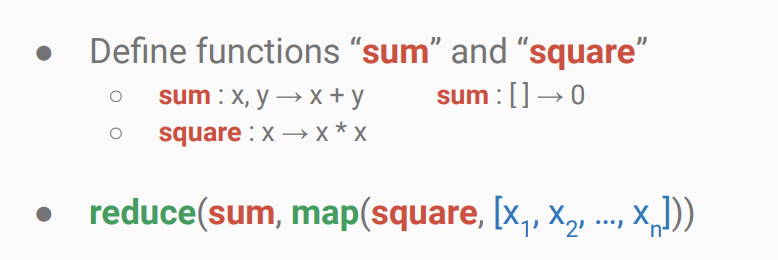
\includegraphics{images/Screenshot 2023-05-08 at 4.51.32 PM.png}
\item the above example, explains a simple example. the map functions maps all elements in a list to its squared values
\item the reduce function holds a variable called sum that is initialized at zero at recursively calls sum on that variable and the next list element
\subsection*{working with map reduce}
\item the programer must write a mapper and reducer function. the more simple the better 
\item the mapper consumers key value pairs as input and outputs intermediate key value pairs
\item the reducer consumes a single key and list of values and produces values for each key. note that in map reduce unlike in functional programming the reducer is not applied recursively
\subsection*{workflow}
\item map phase
\begin{itemize}
    \item distribute data to mappers 
    \item run mappers on chunks of data to get intermediate key value pairs 
\end{itemize}
\item sort shuffle phase
\begin{itemize}
    \item assign a parton of the  intermediate results to each reducer by key
    \item move data from mappers to reducers
\end{itemize}
\item reduce phase
\begin{itemize}
    \item run the reducer call on chunk keys
    \item collect the output 
\end{itemize}
\item make the mapper simple 
\item let the mr frame work route the intermediate results
\item keep the reducer simple if possible 
\subsection*{slido example}
\item 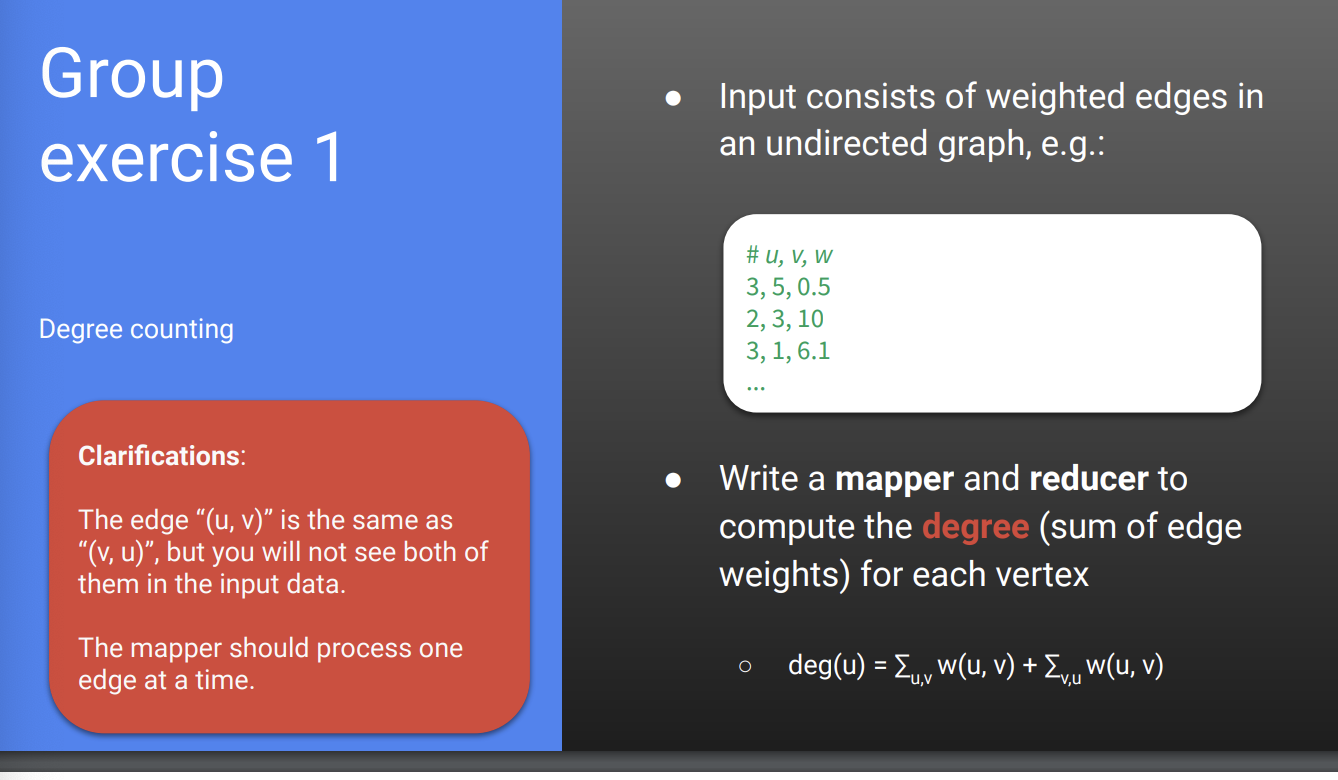
\includegraphics[width=10cm]{images/Screenshot 2023-05-08 at 4.59.20 PM.png}
\item 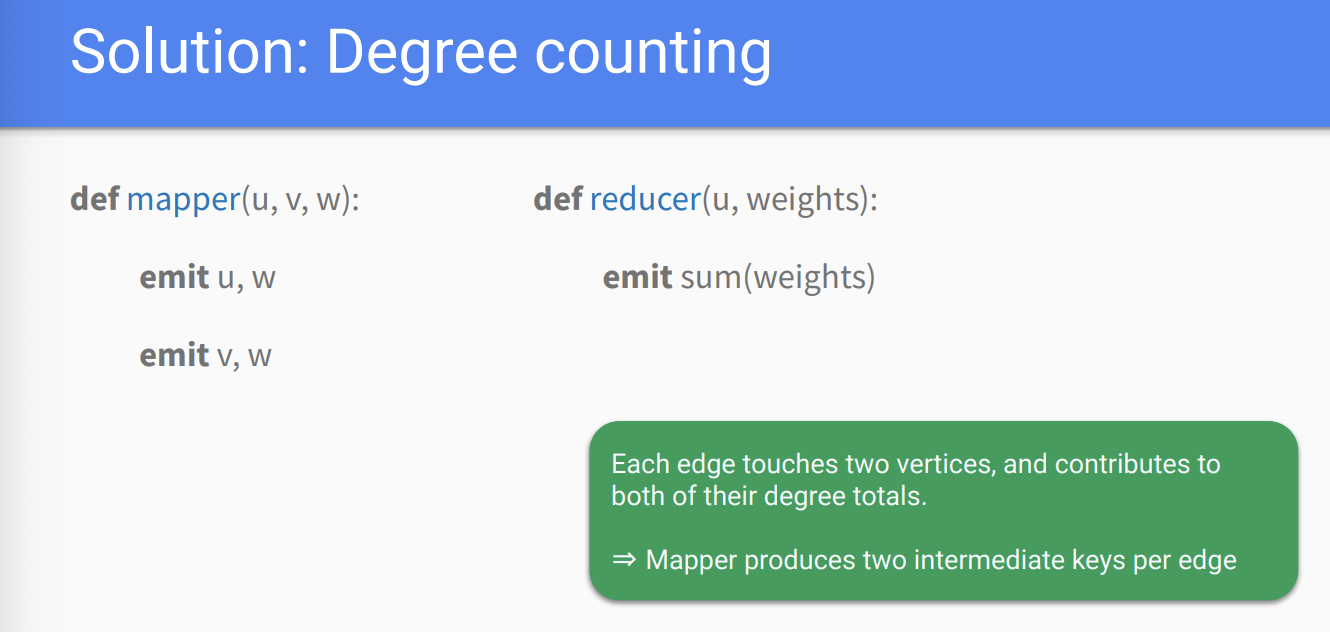
\includegraphics[width=10cm]{images/Screenshot 2023-05-08 at 5.03.47 PM.png}
\item this one is pretty straight forward
\item tips for map reduce 
\begin{enumerate}
    \item do not use floating point keys they don't hash well 
    \item keep map and reduce simple (the sorting is what is optimized so let that do as much work as possible)
    \item compare your algorithm to a simple implementation
\end{enumerate}
\item 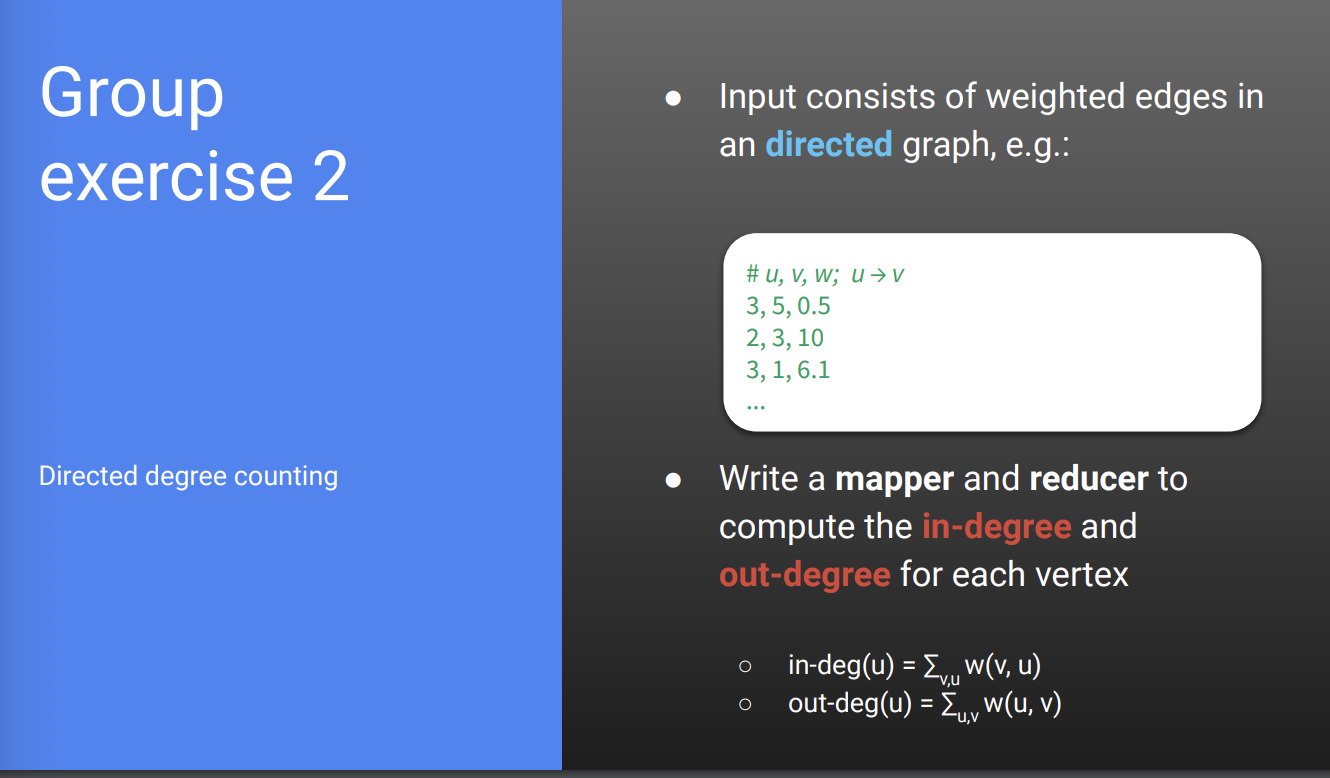
\includegraphics[width=10cm]{images/Screenshot 2023-05-08 at 5.07.04 PM.png}
\item 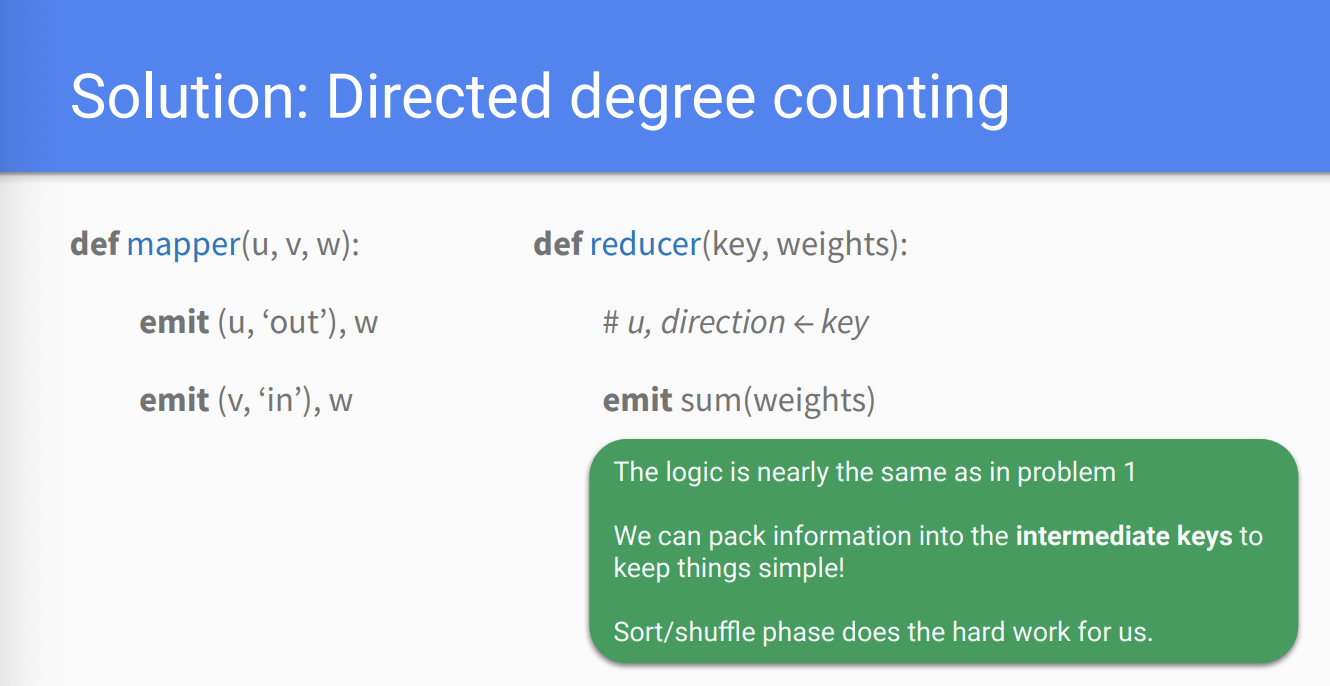
\includegraphics[width=10cm]{images/Screenshot 2023-05-08 at 5.10.06 PM.png}
\item the logic is the same as the last problem the real point is think about changing your keys before making your map program more complex
\subsection*{map reduce in practice}
\item can intermediate outputs be randomly assigned to reducers
\item no we need to make sure all intermediate outputs with the same key go to the same reducer
\item item this leads to key skew
\item so suppose there is are 4 keys and 4 reducers but one key shows up 95\% of the time, then that one reduce worker is doing 95\% of the work this is called \textcolor{purple}{key skew or data skew}
\subsection*{combiners}
\item key skew causes high latency
\item lots of keys also means a lot of communication 
\item we can make the reducer's job easier with \textcolor{green}{combiners} which reduce intermediate key value pairs within the mapper worker, before shuffeling the data
\subsection*{Heuristics for using map reduce well}
\item have fewer mappers than inputs 
\item having fewer reducers than intermediate keys
\item combiners can help but sometimes a more complex map is better 
\item sometimes doing some other sorting stuff can reduce communication 
\section*{criticism of map reduce}
\item map reduce has criticism because it is 
\begin{enumerate}
    \item too low level 
    \item not well implementation
    \item not novel 
    \item missing key DBMS features 
    \item and not compatible with DBMS tools
\end{enumerate}
\item i mean i read the paper 1 4 and 5 are for sure, and i would say probably 2 (due to key skew)
\subsection*{too low level}
\item map reduce does not have schemas, so a programer has to infer them as they work, and there is no garuntee of data consistency 
\item map reduce does not use high level access language like sql which people think is better 
\item there are tools that can be used in tandom with map reduce that can address this 
\subsection*{poor implementation}
\item map reduce does not have the ability to index 
\item is this a major issue? depends on the context 
\subsection*{not novel}
\item map reduce uses old ideas so was not novel but that does not really matter 
\subsection*{missing features }
\item many features from DBMS are not in mpa reduce
\item why are they missing? is this a fair comparison? I am not sure 
\subsection*{lack of DBMS compatability}
\item since this was published this has shifted a lot so not really an issue any more 
\subsection*{why was map reduce so sucessfull}
\item map and reduce are simple abstractions that are powerful  
\item many jobs are only one shot (ie only need to be done once) so it may not be worth the time to build a database infrastructure
\subsection*{map reduce is not a database managment system }
\item but there is some overlap, simple queries can be done in map reduce but not hard queries 
\subsection*{map reduce is not a general comutation engine }
\item maps are reducers are really flexible so a lot can be done with map reduce 
\item it can not however work with iterative or recursive algorithms
\item not can it work with non deterministic functions
\subsection*{no transactions }
\item data base management systems use transactions to make sure data is consistency
\item map reduce does not have transactions but still avoids these issues by having data be immutable, and require programs to be deterministic
\item it has error tolerence if a node fails we can re assign idle workers to do its task 
\subsection*{real issues with map reduce}
\item key skew so there are latency and scheduling issues 
\item we store intermediate results in many files 
\item not all tasks fit neatly into map reduce including non deterministic tasks, iterative algorithms or recursive algorithms
\item cant do visualizations 
\subsection*{what is the role of map reduce today}
\item map reduce is good for large batch jobs that run once or infrequently 
\item like data transformations or feature extaction 
\subsection*{why is map reduce studied}
\item it is important for the development of big data tools 
\item map and reduce functions are a good way to break down problems 
\item the hadoop eco system is much bigger than map reduce 
\item there are still legacy code bases run in map reduce 
\end{itemize}
\end{document}
